%%This is a very basic article template.
%%There is just one section and two subsections.
%\documentclass[12pt, a4paper, notitlepage]{article}
\documentclass[12pt, a4paper]{article}

\usepackage[brazil]{babel}    % dá suporte para os termos na língua portuguesa do Brasil
\usepackage[utf8]{inputenc} % ou latin1 dá suporte para caracteres especiais como acentos e cedilha
\usepackage[T1]{fontenc}      % Lê a codificação de fonte T1 (font encoding default é 0T1).
\usepackage[center,small]{caption} % legendas centralizadas e pequenas

%\usepackage{ae}               % Fonte "Almost European"
%\usepackage{lmodern}        % Fonte "Latin Modern", experimente no lugar de ae
%\usepackage{times}          % Fonte "Times New", experimente no lugar de ae
%\usepackage{helvet}

%\renewcommand*\familydefault{\sfdefault} %% Only if the base font of the


\usepackage{indentfirst}       % indenta os primeiros parágrafos
\usepackage{amssymb,amsmath}   % simbolos matemáticos providos pela AMS
%\usepackage[pdftex,dvipdfm]{graphicx}
% para inclusão de figuras (png, jpg, gif,bmp)
\usepackage{graphicx}          % figuras gráficas
\usepackage{geometry}
%\usepackage{layouts} 
\usepackage{color}             % para letras e caixas coloridas
%\usepackage{makeidx}           % índice remissivo
\usepackage{a4wide}            % correta formatação da página em A4
\usepackage{setspace}          % para a distância entre linhas

\usepackage{longtable} % tabelas longas

% Formatação ============================================================================
%\geometry{paperwidth=21cm,paperheight=29.7cm,
%left=3.5cm,right=3.5cm,top=2.5cm,bottom=2.5cm}
\geometry{paperwidth=21cm}
\geometry{paperheight=29.7cm}
\geometry{left=3.5cm}
\geometry{right=3.5cm}
\geometry{top=2.5cm}
\geometry{bottom=2.5cm}
\geometry{headheight=15pt}
\geometry{headsep=10mm}                  % espaço entre parágrafo e cabeçalho
\geometry{footskip=10mm}                 % espaço entre parágrafo e rodapé
% ---------------------------------------------------------------------------------------
\setlength{\parindent}{1.5cm}             % indentação do parágrafo
\setlength{\parskip}{6pt}                % espaço entre parágrafos
\setlength{\abovecaptionskip}{3pt}       % espaço entre legenda e tabela ou gráfico
%\setlength{\belowcaptionskip}{1pt}       % espaço entre legenda e tabela ougráfico 
\setlength{\doublerulesep}{1pt}          % espaço entre linhas duplas de uma tabela
%\usepackage[num,overcite]{num-abnt}
%\citebrackets[]


%\usepackage{listings}
%\renewcommand{\lstlistingname}{Listagem}
%\renewcommand{\lstlistlistingname}{Lista de Listagens}


\newcommand{\remove}[1]{}

\hyphenation{tra-zen-do Bra-sil}

\begin{document}

\title{Ferramenta de Suporte a Experimentação em Documentos HTML}

\maketitle


\section{Introdução}

%o que é um problema em aberto? não resolvido? não solucionado? 

Existem diversos problemas não solucionados que envolvem a
recuperação, indetificação e segmentação de 
informação de documentos HTML. Por serem referentes a documentos disponíveis
na Web, normalmente, esses problemas demandam a
experimentação em conjuntos de controle para que se possa avaliar o
comportamento da solução proposta antes de coloca-la em produção.

% voce esta usando muito 'diversas vezes', 'em sua maioria'
% vc escreve de uma forma vaga: olhe o pargrafo anterior 'diversos problemas'. quais sao esses? olhe esse paragrafo: 'problemas com codificação': existe mais de um problema relacionado a codificação? ou codificação é um problema só?
% penultima linha do proximo paragrafo: vc tinha escrito 'foge ao dominio'. 

A experimentação em documentos HTML pode ser uma tarefa trabalhosa, pois
para atacar o problema proposto é necessário antes enfrentar diversas
barreiras para que o documento HTML possa ser carregado em memória e
analisado. Por exemplo, diferentes codificações de caracteres ou má geração do
HTML são esperados dentre os documentos da Web, o que pode 
exigir profundo conhecimento de aspéctos como a costrução da linguagem ou
tabelas de codificação que, em grande maioria, fogem do domínio da tarefa
principal desejada.

%minha preocupação nao é com o texto deste projeto final e sim tentar melhorar sua escrita geral, visando a dissertacao. observe como inicio desse paragrafo está muito vago 'apos sanar TODOS os problemas...' quais sao esses todos os problemas? foram apenas os 2 acima? se vc teve de se preocupar com N problemas, eu creio que seja necessário pelo menos listar (em tópicos mesmo) quais sao esses N problemas.

%"surgem novos desafios que poderia ser evitada" concordancia em genero e em numero erradas.

Após sanar alguns dos problemas referentes ao tratamento dos documentos
HTML, surgem novos desafios, que mesmo tendo um vínculo maior com a tarefa
desejada, poderiam ser evitados. O aspécto de como guardar o conjunto
resposta e de como avaliar o resultado que foi obtido é enfrentado por
todos que desejam realizar experimentos com documentos HTML. Porém em
grande parte dos trabalhos apresentados, a abordagem é semelhante, o que
sugere espeço para a criação de um conjunto de ferramentas públicas que
facilite também a tarefa de anotar e avaliar os resultados.

O cenário descrito nos paragrafos anteriores é encontrado ao se estudar 
trabalhos relacionados a recuperação de informação e segmentação em documentos
HTML. Com isso, este trabalho propõe uma ferramenta para
facilitar futuras tarefas de experimentação em documentos HTML.

As seções seguintes apresentarão os modelos e caracteristicas
necessárias para uma ferramenta de suporte à experimentação em
documentos HTML.

\section{Modularização da Ferramenta}

\begin{figure}[htb]
  \begin{center}
  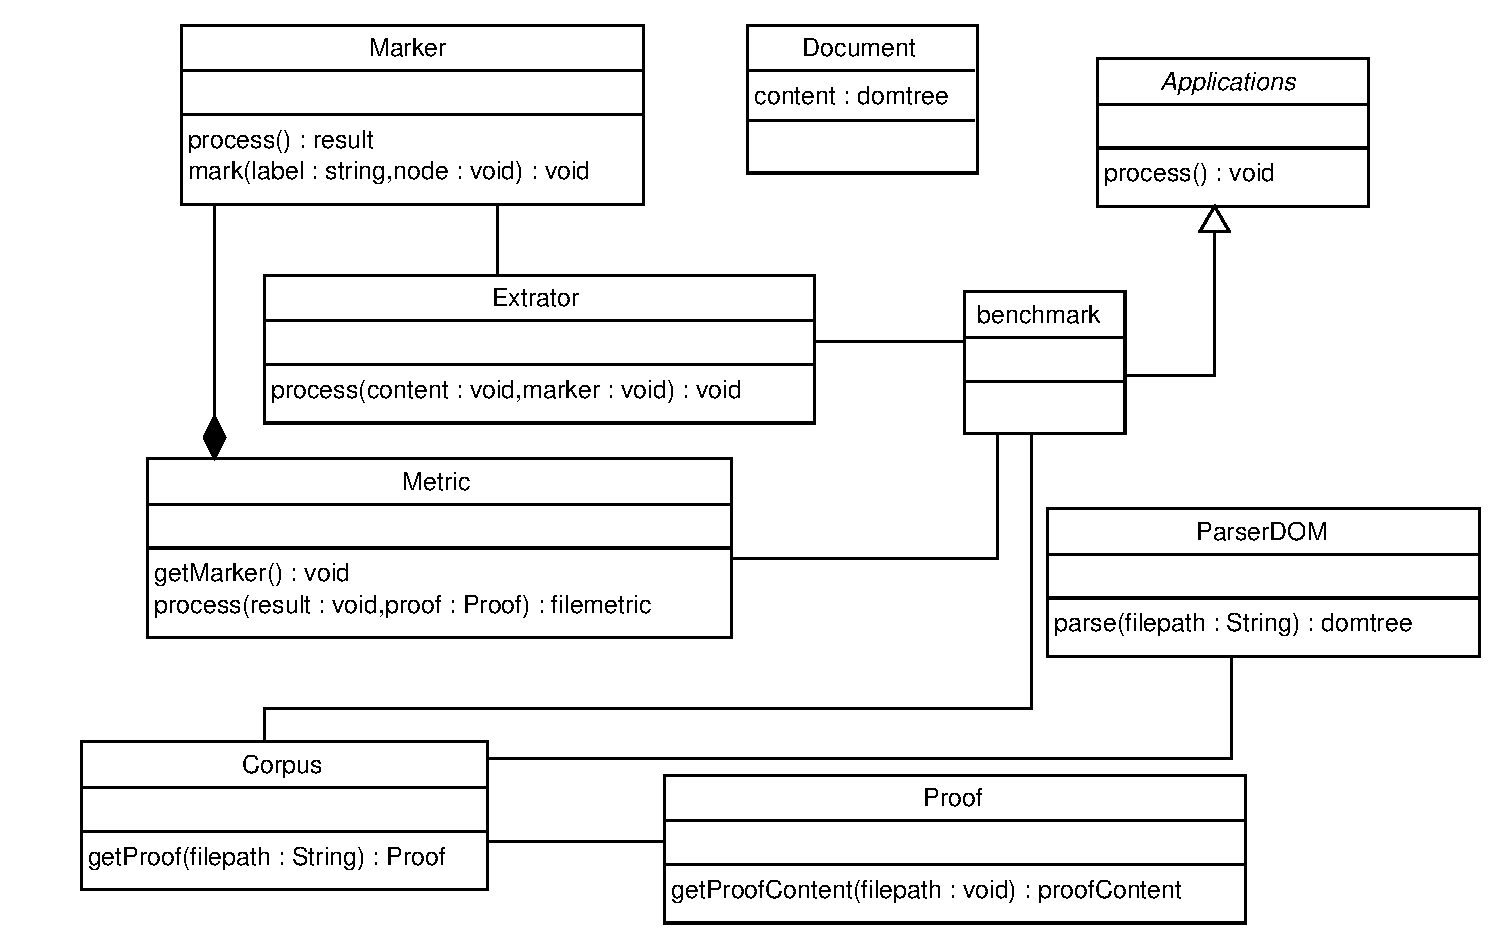
\includegraphics[width=13cm]{img/classes.eps}
  \caption{Diagrama de classes da ferramenta}
  \label{classes}
  \end{center}
\end{figure}

% Le esse paragrafo de novo. Tah faltando pontuacao.

Observando os passos necessários para que seja possível o 
desenvolvimento de uma solução de experimentação, fica evidente a
necessidade de um módulo capaz de corrigir problemas de
codificação e má formação nos documentos HTML. Além
disso, é necessário também uma estrutura em memória que permita a
manipulação do documento por algoritmos.
O módulo que atende essas necessidades é chamado de Parser, sendo 
descrio a seguir:

\begin{verbatim}
- Parser: 
  - ForceEncode:
    Normaliza a codificação de um documento para
    UTF-8.
  - Santizer:
    Verifica a corretude do documento HTML e
    corrige alguns erros e problemas comulmente
    encontrados.
  - ParserDOM:
    Transforma o documento em uma estrutura em
    memória DOM, essa estutura é recomendada
    para a representação de documentos HTML
    em memória pela W3C.
\end{verbatim}

%Nao entendi.
Com o documento HTML em memória e disponível para a execução de rotinas
sobre sua estrutura. A forma como as rotinas irão guardar seus resultados
é importante, pois determinará todo o processo de geração de resultados
e avaliação. Com isso, descrevemos o módulo de ``anotação'' e a interface
que todas as rotinas, denominadas extratores, devem atender.

Existe uma peculariedade com a modelagem adotada, pois a forma de marcar
o resultado influencia como esse resultado poderá ser avaliado, porém
essa dependecia será descrita junto com o módulo de avaliação.

\begin{verbatim}
- Marcadores:
  Armazena nós em rótulos para que eles possam ser
  organizados ou segmentados.

- Extratores:
  Procura por elementos, nós ou conjunto de nós, que
  atendendam as especificações de um rótulo e os marca,
  passando para o marcador o rótulo e o nó que deve
  ser marcado pelo referido rótulo.
\end{verbatim}

Os módulos descritos fornece um conjunto de
funcionalidades que proporcionam a aplicação, ou seja, a colocação em
prática da solução encontrada,
porém como o objetivo da ferramenta é proporcionar um ambiente
de experimentação, são necessários módulos para realizar a tarefa de experimentação.

% porque é mt importante?
A capacidade de avaliar os algoritmos, ou soluções, propostos é
importante, pois permite que se tenha a visão de que tipo de resultado
esta sendo gerado. Por isso, o módulo de avaliação fornece o conjunto de
regras para que o resultado obtido possa ser mensurado e retornado como
informação estatística. As formas de avaliar são diretamente
relacionadas a forma que o resultado foi armazenado. Assim, para cada
avaliador existe um marcador disponível, pois esse marcador armazena a
solução no formato adequado para ser posteriormente avaliado.

%Acho que esse foi o melhor paragrafo.

Além de um marcador, o avaliador necessita também de uma fonte de
informação correta, denominada gabarito. Esse gabarito fornece um
conjunto de informação, no mesmo formato que o conjunto armazenado pelo
marcador, para que seja possível o cruzamento de informação para a
avaliação. Um formato básico que atende as principais tarefas de
identificação em páginas HTML é fornecido como base junto a ferramenta.

\begin{verbatim}
- Avaliador:
  Recebe os rótulos, junto aos conjunto de nós
  que pertencem a eles, e também o gabarito para
  quantificar a qualidade do extrator.

- Gabarito: 
  Armazena os rótulos, junto ao conjunto de nós
  de cada rótulo, para que os extratores possam
  ser avaliados.
\end{verbatim}

%descrevemos uma estrutura que descreve: RUIM.
% e eu nao entendi o que é o corpus. é a estrura que descreve esse conjunto ou é o conjunto?
% esta repetindo muito as palavras.

A experimentação normalmente ocorre sobre um grande conjunto de
documentos, por esse motivo foi criada uma estrutura que descreve esse
conjunto, denominado corpus. O corpus descreve um conjunto de
documentos, informando a natureza dos documentos, o tipo de gabarito que
pode ser obtido dos documentos e para quais tarefas esses documentos são
interessantes.

\begin{verbatim}
- Corpus: 
  Conjunto de documentos, junto aos seus gabaritos.
  Os corpus são descritos por um arquivo de
  configuração que especifica o tipo de gabarito
  que esse corpus pode produzir e quais as tarefas
  que ele pode ser utilizado.
\end{verbatim}

% ela quem? 
Para utilizar esses módulos podem ser implementadas aplicações que
utilizam o que é mais interessante. Um bom exemplo de aplicação
é a geração de um relatório de desempenho (Benchmark) para o conjunto de
extratores e corpus. Atualmente, o benchmark é a unica aplicação
disponível junto a ferramenta, pois essa é uma necessidade direta para a
experimentação. A seguir é apresentado um diagrama de sequência para
exemplificar a utilização da ferramenta.

\begin{figure}[htb!]
  \begin{center}
  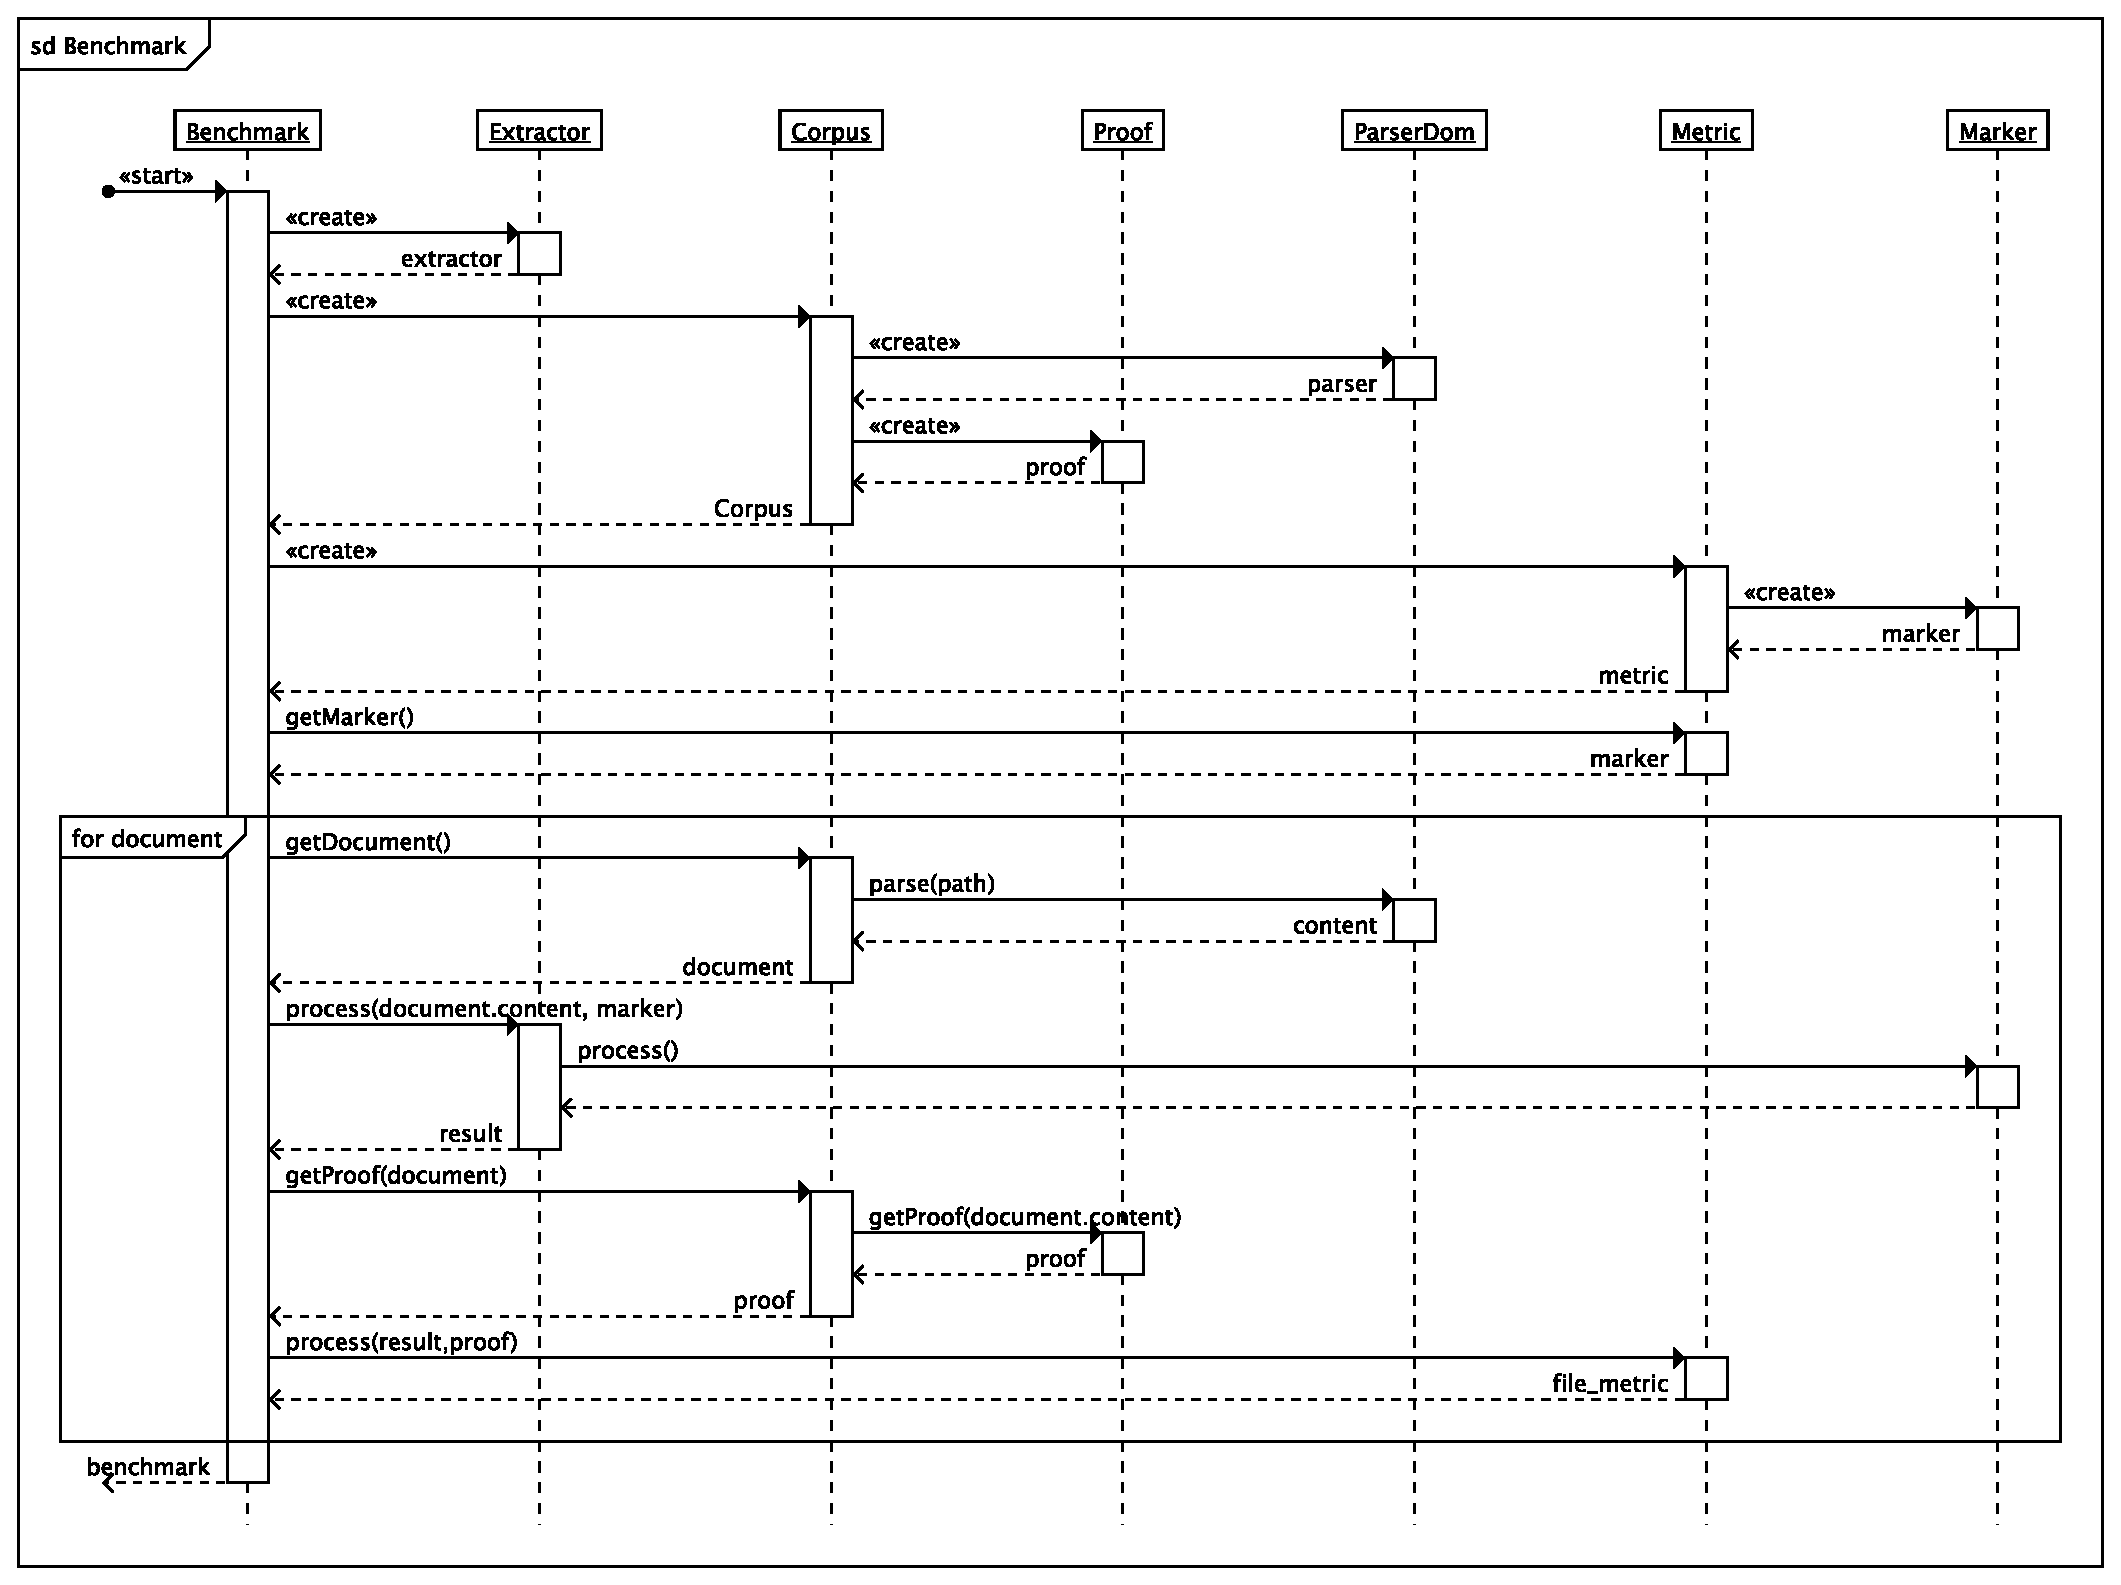
\includegraphics[width=14cm]{img/fastbenchmark.eps}
  \caption{Diagrama de sequência do aplicação Benchmark}
  \label{sequencia}
  \end{center}
\end{figure}

\section{Acompanhamento do Desenvolvimento da Ferramenta}

%- mini-acompanhamento da execução: seqüência de tarefas de desenvolvimento utilizadas junto com estatísticas de tempo e esforço por tarefa.
\begin{enumerate}
\item Definição da Tarefa: 1 de agosto a 30 de agosto. \\
Inicialmente foi realizada uma busca pelos trabalhos relacionados à
extração de elementos e marcação em páginas Web para engrandecer o
conhecimento sobre a área, melhorando a capacidade de entendimento
sobre o problema.

\item Modelagem do Problema: 1 de setembro a 15 de setembro. \\ 
Após conhecer bem o problema de segmentação e marcação de elementos em
documentos HTML, a modelagem de uma ferramenta de apoio se tornou possível.
Durante o processo de modelagem, foram estabelecidos os limites e as
necessidades de uma ferramenta a experimentação em documentos HTML.

\item Impementação da Ferramenta e Testes: 15 de setembro a 30 de
novembro. \\
Durante o mês de setembro, outubro e novembro foi realizada a
codificação da ferramenta modelada. Durante esse tempo, também foram
desenvolvidos os testes unitários para garantir a qualidade do
desenvolvimento da aplicação. Além do desenvolvimento da ferramenta de
suporte, também foi realizada a tentativa de resolver uma tarefa de
segmentação. Essa tarefa será detalhada mais adiante no texto, assim como
seus resultados.

\item Documentação de usuário e relatório: 30 de novembro a 15 de
dezembro. \\
Os últimos 15 dias de projeto foram utilizados para a elaboração deste
documento e também para a criação da documentação para usuários,
tornando a ferramenta fácil de ser utilizada por qualquer um que
queira realizar experimentos em documentos HTML de forma semelhante a
que a ferramenta atende, ou seja, experimentação de problemas de
segmentação ou detecção de elementos em documentos HTML.
\end{enumerate}

\section{Código Fonte}

%Essa secao está melhor.

Para a codificação da ferramenta foi escolhida a linguagem script
Python. Sua facilidade de prototipação e programação foram pontos
positivos para essa escolha.

Para tornar o código claro e padronizado foram utilizadas as
recomendações de codificação da empresa Fast.
Isso porque, as normas apresentadas são próximas as utilizadas pelos 
próprios módulos disponibilizados nas bibliotecas padrões e, além disso,
esclarecem pontos que muitas vezes ficam dúbios em outros manuais de 
recomendações para codificação em Python. Porém,
  o documento contendo as recomendações e regras não
  poderá ser anexado por causa dos termos de sigilo. 

Todo o código esta comentado no formato recomendado pelo manual de
referência de Python e o  módulo de geração de documentação automático
PyDoc foi utilizado, gerando a documentação em formato HTML. Para a
documentação do código também foi adotado, como adendo, o padrão de 
descrição de comentário recomentado pela empresa Fast.

\section{Validação e Testes}

Para verificar o funcionamento da ferramenta e validar a modelagem apresentada,
a tarefa de identificação de tabelas genuinas foi escolhida. Utilizando a
Ferramenta de Experimentação em Documentos HTML foi implementada uma abordagem
simplificada a proposta em \cite{LGZ2003}. Mesmo não obtendo bons resultados
para a tarefa, o objetivo foi alcançado, já que a ferramenta proporcionou a
rápida codificação e experimentação da tarefa. Esses resultados estão
disponíveis no Anexo \ref{ritg} e um fragmento do corpus utilizado está disponível junto ao código para a realizações de testes pelo usuário.

Foi utilizado o framework de teste unitários fornecido pela distribuição
oficial do Python \cite{UTest}. Os módulos foram testados, buscando a verificação
da corretude do código e também foram criados testes para verificar a
API das classes importantes para a ferramenta.

Os testes e todos os logs podem ser verificados no Anexo \ref{testes}. Esses testes
também se encontram junto ao código, sendo eles nomeados como
test\_<nome\_do\_arquivo>.py e podem ser executados separadamento como
um scripts Python.

A cobertura do código por testes foi programada a partir do modelo de
sequência da aplicação ``Benchmark'' que descreve o principal uso da
ferramenta. Outros casos também foram verificados para garantir que
módulos de suporte, como o parser DOM ou algorítmos clássicos como
distáncia de ediçao, DFS, LLC estão corretamete
implementados.

\section{Documentação do Usuário}

A documentação para utilização das aplicações existentes na ferramenta
se encontram junto ao código e são apresentadas quando o usuário
solicita ajuda (-help) pela linha de comando. Essa documentação foi
criada utilizando a biblioteca optparser, também disponibilizada pela
distribuição oficial de Python. A documentação para usuário existente em
código foi adicionada e este documento no Anexo \ref{userdoc}.


\section{Conteúdo do CD}

O CD-ROM engtregue, onde este documento pode ser encontrado, contêm
todos os arquivos fonte e documentos necessários para o entendimento e
utilização da ferramenta. Também é fornecido um pequeno conjunto de
documentos onde a tarefa de detecção de tabela genuida pode ser
executada e os resultados analizados utilizando a aplicação de Benchmark.

A Estrutura de diretórios do código fonte, que pode ser encontrada na
pasta source, é a seguinte:

\begin{verbatim}
|-- source
  |-- README.txt 
  |-- __init__.py
  |-- apps
  |   |-- __init__.py
  |   |-- benchmark.py
  |   |-- config_example.cnf
  |   |-- configurator.py
  |   |-- fastbenchmark.py
  |   |-- test_.py
  |   |-- test_benchmark.py
  |   `-- test_configurator.py
  |-- corpus.py
  |-- extractors
  |   |-- __init__.py
  |   `-- distancebypair
  |       |-- __init__.py
  |       |-- coloring.py
  |       |-- distancebypairbase.py
  |       |-- node.py
  |       |-- table.py
  |       `-- test_node.py
  |-- markerbase.py
  |-- markercoloring.py
  |-- metricbase.py
  |-- metrictables.py
  |-- tablesproof.py
  |-- test_corpus.py
  `-- utils
      |-- __init__.py
      |-- distances.py
      |-- dynamicimport.py
      |-- forceencode.py
      |-- parsedom.py
      |-- sanitizer.py
      |-- test_distances.py
      |-- test_dynamicimport.py
      |-- test_forceencode.py
      `-- test_parsedom.py
\end{verbatim}

Na pasta pydoc pode ser encontrado a documentação gerada automaticamente
a partir do código.

\begin{verbatim}
|-- pydoc
  |-- benchmark.html
  |-- configurator.html
  |-- corpus.html
  |-- distancebypairbase.html
  |-- distances.html
  |-- dynamicimport.html
  |-- fastbenchmark.html
  |-- forceencode.html
  |-- markerbase.html
  |-- markercoloring.html
  |-- metricbase.html
  |-- metrictables.html
  |-- node.html
  |-- sanitizer.html
  |-- table.html
  |-- tablesproof.html
  |-- test_benchmark.html
  |-- test_configurator.html
  |-- test_corpus.html
  |-- test_distances.html
  |-- test_dynamicimport.html
  `-- test_parsedom.html

\end{verbatim}

Na pasta corpus, o sample para a execução e teste do benchmark pode ser
encontrado:

\begin{verbatim}
|-- corpus
    |-- file0.html 
    |
    `-- filen.html
\end{verbatim}

Para exemplificar o resultado de um Benchmark em um conjunto real de
documentos e o tempo de execução, um corpus utilizado em estudos da área,
foi adicionado ao CD-ROM a pasta experimento.

\begin{verbatim}
|-- experiments
  |-- benchmark100docs
  |-- benchmark300docs
  |-- benchmark600docs
  |-- out100docs.out
  |-- out300docs.out
  `-- out600docs.out
\end{verbatim}

\appendix

\section{Anexos}
\subsection{Manual do Usuário}
\label{userdoc}

\begin{verbatim}
Usage: benchmark.py [options] <extractor> <cPath>
<extractor> User an module name [DistanceByPair.Coloring
            | DistanceByPair.Table]
<cPath>     Corpus path 

Options:
  -h, --help            show this help message and exit
  -o OUTPUT, --output=OUTPUT
                        Create and redirect stdout to file
  -l LIMIT, --limit=LIMIT
                        Set limit to hierarchical corpus 
                        (default use no hierarchical corpus)
                         or -1 to directory with files
                        (use -l < -1 to limit # of files
  -c CONFIG, --config=CONFIG
                        Configuration file to set Marker, 
                        ProofClass, and Marker, if omited
                        fastbenchmark use config\_example.cnf
                        (make sure provided corpus is
                        ProofTable based)

\end{verbatim}

\subsection{Resultados da Identificação de Tabelas Genuidas}
\label{ritg}

\subsection{Log dos Testes Unitários}
\label{testes}

Log Geral:
\begin{verbatim}
nosetests
.................
----------------------------------------------------------
Ran 18 tests in 8.000s

OK

\end{verbatim}

Log passo a passo:
\begin{enumerate}

\item Teste Distancias

\begin{verbatim}
Test: utils.distances

 - Test: utils.distances.stringDistance()
.
------------------------------------------------------------
Ran 1 test in 0.000s

OK
\end{verbatim}

\item Teste Intanciação Dinamica

\begin{verbatim}
Test: utils.dynamicimport
.
------------------------------------------------------------
Ran 1 test in 0.000s

OK
\end{verbatim}

\item Teste Force Encode

\begin{verbatim}
Test: utils.forceencode
   - Test: utils.parsedom._convertStringToUTF8()
.
------------------------------------------------------------
Ran 1 test in 0.000s

OK
\end{verbatim}

\item Teste ParseDom
\begin{verbatim}
Test: utils.parsedom
   - Test: utils.parsedom.parse()
.
--------------------------------------------------------------
Ran 1 test in 0.001s

OK
\end{verbatim}

\item  Teste Node From Distance By Pair

\begin{verbatim}
Test: distancebypair.node
body
..
---------------------------------------------------------------
Ran 2 tests in 0.002s

OK
\end{verbatim}

\item Teste Configurator

\begin{verbatim}
Test: apps.configurator
   - Test apps.configurator.marker()
.  - Test apps.configurator.metric()
.  - Test apps.configurator.proof()
.  - Test apps.configurator()
.
---------------------------------------------------------------
Ran 4 tests in 0.001s

OK
\end{verbatim}

\item Teste benchmark

\begin{verbatim}
Test: apps.configurator
encoder error0 {'table': [0, 2, 4]}
1 {'table': [1, 1, 12]}

total
{'table': [1, 3, 16]}

key recall  precision
{'table': [0.33333333333333331, 0.0625]}
encoder error0 {'table': [0, 2, 4]}
1 {'table': [1, 1, 12]}
2 {'table': [0, 1, 20]}
3 {'table': [3, 3, 24]}
4 {'table': [23, 23, 69]}
5 {'table': [0, 0, 72]}
6 {'table': [0, 0, 78]}
7 {'table': [1, 1, 84]}
8 {'table': [0, 0, 93]}
9 {'table': [0, 0, 96]}

total
{'table': [28, 31, 552]}

key recall  precision
{'table': [0.90322580645161288, 0.050724637681159424]}
.
-------------------------------------------------------------
Ran 2 tests in 7.064s

OK
\end{verbatim}

\item Teste Corpus

\begin{verbatim}
t: apps.configurator
   - Test geral
path /home/iamjabour/workspacePessoal/tese/corpus/machine
_learning_tableextraction_paper2/webtablegrnd/html
parser <eri.utils.parsedom.ParseDom object at 0x209b450>
proof <eri.tablesproof.TablesProof object at 0x209b4d0>
documents len 1393
path /home/iamjabour/workspacePessoal/tese/corpus/machine
_learning_tableextraction_paper2/webtablegrnd/html_desc
parser <eri.utils.parsedom.ParseDom object at 0x209bd50>
proof <eri.tablesproof.TablesProof object at 0x209b510>
documents len 1393
.path /home/iamjabour/workspacePessoal/tese/corpus/machine
_learning_tableextraction_paper2/webtablegrnd/html
parser <eri.utils.parsedom.ParseDom object at 0x209b510>
proof <eri.tablesproof.TablesProof object at 0x209bd50>
documents len 1393
<eri.corpus.Doc instance at 0x209a560> 0 /home/iamjabour/
workspacePessoal/tese/corpus/machine_learning_table
extraction_paper2/webtablegrnd/html/industry.ebi.ac.uk.w2h
.Doc.help.mangpage.html <libxml2dom.Document object at 
0x209bcd0>
{'table': [<libxml2dom.Node object at 0x21114d0>, 
<libxml2dom.Node object at 0x2111710>]}
<eri.corpus.Doc instance at 0x209a488> 1 /home/iamjabour/
workspacePessoal/tese/corpus/machine_learning_table
extraction_paper2/webtablegrnd/html/www.ovonic.com.news.
Nov14_2000.html <libxml2dom.Document object at 0x209b450>
{'table': [<libxml2dom.Node object at 0x2111350>]}
<eri.corpus.Doc instance at 0x209a440> 2 /home/iamjabour/
workspacePessoal/tese/corpus/machine_learning_table
extraction_paper2/webtablegrnd/html/news.cnet.com.news.
0-1005-200-1507039.html <libxml2dom.Document object at 
0x209bcd0>
{'table': [<libxml2dom.Node object at 0x2113510>]}
<eri.corpus.Doc instance at 0x209a5a8> 3 /home/iamjabour/
workspacePessoal/tese/corpus/machine_learning_table
extraction_paper2/webtablegrnd/html/www.dieoff.org.page114.
htm <libxml2dom.Document object at 0x209b450>
{'table': [<libxml2dom.Node object at 0x2116890>, 
<libxml2dom.Node object at 0x2116950>, 
<libxml2dom.Node object at 0x2116c10>]}
<eri.corpus.Doc instance at 0x209a248> 4 /home/iamjabour/
workspacePessoal/tese/corpus/machine_learning_table
extraction_paper2/webtablegrnd/html/www.microsoft.com.Open
Type.OTSpec.base.htm <libxml2dom.Document object at 0x209bcd0>
{'table': [<libxml2dom.Node object at 0x21198d0>, 
<libxml2dom.Node object at 0x2119bd0>, 
<libxml2dom.Node object at 0x2119f90>, 
<libxml2dom.Node object at 0x211a310>,
<libxml2dom.Node object at 0x211a5d0>, 
<libxml2dom.Node object at 0x211abd0>, 
<libxml2dom.Node object at 0x211ae90>]} 
<eri.corpus.Doc instance at 0x209a488> 5 /home/iamjabour/
workspacePessoal/tese/corpus/machine_learning_table
extraction_paper2/webtablegrnd/html/directory.google.com.Top.
Science.Technology.Electronics.Test.Programming_Services.
index.html <libxml2dom.Document object at 0x209b450>
{'table': []}
<eri.corpus.Doc instance at 0x209a440> 6 /home/iamjabour/
workspacePessoal/tese/corpus/machine_learning_table
extraction_paper2/webtablegrnd/html/www.washingtonpost.com.wp-
dyn.politics.elections.2000.index.html <libxml2dom.Document 
object at 0x209bcd0>
{'table': []}
<eri.corpus.Doc instance at 0x209a488> 7 /home/iamjabour/
workspacePessoal/tese/corpus/machine_learning_table
extraction_paper2/webtablegrnd/html/www.cnn.com.2001.US.01.25
.power.woes.gov.index.html <libxml2dom.Document object 
at 0x209b5d0>
{'table': [<libxml2dom.Node object at 0x2119210>]}
<eri.corpus.Doc instance at 0x209a440> 8 /home/iamjabour/
workspacePessoal/tese/corpus/machine_learning_table
extraction_paper2/webtablegrnd/html/chicagosports.com.notfound
.index.html <libxml2dom.Document object at 0x209b450>
{'table': []}
<eri.corpus.Doc instance at 0x209a5a8> 9 /home/iamjabour/
workspacePessoal/tese/corpus/machine_learning_table
extraction_paper2/webtablegrnd/html/www2.gol.com.users.isett.
stock.pages.philippines.html <libxml2dom.Document object 
at 0x209b5d0>
{'table': []}
.path /home/iamjabour/workspacePessoal/tese/corpus/machine_
learning_tableextraction_paper2/webtablegrnd/html
parser <eri.utils.parsedom.ParseDom object at 0x209bdd0>
proof <eri.tablesproof.TablesProof object at 0x209bd50>
documents len 1393
.
-----------------------------------------------------------
Ran 3 tests in 0.362s

OK
\end{verbatim}
\end{enumerate}

\bibliographystyle{alpha}
\bibliography{bib}
\end{document}
